\documentclass[a4paper,11pt,fleqn]{article}
\usepackage[inner=2.5cm,outer=2.5cm,top=4cm,bottom=3.5cm]{geometry}
\usepackage[T1]{fontenc}
\usepackage[utf8]{inputenc}
\usepackage[french]{babel} 
\usepackage{enumitem}
\usepackage{eurosym}
\usepackage{amsmath}
\usepackage{fancyhdr}
\usepackage{graphicx}
\usepackage{amsmath}
\usepackage{float}
\usepackage{hyperref}
\pagestyle{fancy}

\renewcommand{\headrulewidth}{1pt}
\fancyhead[C]{} 
\fancyhead[L]{PROJET TSP}
\fancyhead[R]{VALDES-ALONZO SOGHAIER}
\setlength{\headheight}{23pt}

\title{\underline{Projet Mathématiques - Informatique}}
\author{Gabriel VALDES-ALONZO\\ Sami SOGHAIER  \\\\ Licence 3 - Mathématiques-Informatique \\ Maria Raquel URENA PEREZ }
\date{Juin 2025}

\begin{document}
\pagenumbering{gobble}
\maketitle
\begin{center}
    
\includegraphics[scale=0.7]{index.png}
\end{center}

\newpage
\pagenumbering{arabic}

\section*{\underline{Introduction}}
Le problème du voyageur de commerce \cite{book:TSP,chap:TSP} (Traveling Salesman Problem en anglais) est un problème classique d’optimisation combinatoire : le problème consiste à trouver le plus court chemin passant une seule fois par une liste de $n$ villes définies, et revenant au point initial.

Le TSP a diverses applications dans plusieurs domaines comme la logistique, séquençage d'ADN, manufacture, et autres. Chaque problème composé d'un ensemble que doit être rempli dans un ordre particulier pourrait être pensé comme le problème TSP, où on cherche un chemin moins coûteux. Le problème peut être résolu exactement si tous les chemins entre villes sont analyses et comparés, mais la quantité de chemins à vérifier augmente rapidement, ce qu'est connu comme un problème NP-Difficile.

Dû à son coût, des algorithmes sont proposés pour trouver des solutions approximatives que peuvent être optimales ou pas, mais qui résolut le problème rapidement. Dans ce travail, seulement la version symétrique de l'algorithme sera analyse. Cela veut dire que les distances considérées entre villes sont égales dans les deux sens. Les villes sont aussi considérées toutes interconnectés, donc il existera toujours une connexion directe entre une ville et l'autre.

Le travail suivant a été réparti de la façon suivante : chaque personne a pris deux algorithmes à implémenter. L'heuristique du plus proche voisin ainsi que 2-opt sont une continuité, comme l'heuristique d'Insertion qui fonctionne avec le recuit simulé. En ce qui concerne le rapport, il a été écrit en développant chacun les parties respectives et en faisant les analyse ensemble.

Dans les prochaines sections, on procédera ensuite à l’analyse des résultats et puis on finira par conclure en comparant les résultats et regardant les perspectives à futur.

Divers outils ont été utilisés pour travailler sur le rapport :
\begin{itemize}[noitemsep,topsep=5pt]
    \item Overleaf : pour rédiger le rapport et travailler ensemble en temps réel,
    \item Notebook : pour rédiger le notebook jupyter,
    \item VSCode : pour travailler sur le code du projet,
    \item Github : pour stocker et échanger les différents supports.
\end{itemize}

Le dépôt Github peut être consulté sur le lien 

\noindent \url{https://github.com/grvaldes/EADS-projet-mathematique}.

\section*{\underline{Heuristiques implémentés}}
Dans le contexte de ce travail sur le TSP,  on va mettre en pratique des heuristiques afin d’apporter des solutions qui soient le plus correctes possible en minimisant le temps de calcul.
Les heuristiques analysés sont las suivantes :
\subsection*{Voisins Plus Proches}
L'heuristique VPP \cite{article:nearest}, aussi connu par son nom en anglais Nearest Neighbors, est un des algorithmes plus simples et intuitives pour résoudre le TSP. Comme son nom le dit, ;étant donnée une ville de départ quelconque (choisi arbitrairement), on cherche entre tous les villes voisines laquelle qui est à la moindre distance. Une fois dans cette ville, on la marque comme visité et continue en cherchant la ville la plus proche encore pas visité. On répète cette procédure jusqu'à visiter toutes les villes dans le réseau. La complexité de cet algorithme est exactement $\mathcal{O}(n^2)$ (avec $n$ la quantité de villes), car pour chaque ville il faut vérifier la distance avec chaque voisin.

\begin{figure}[H]
    \centering
    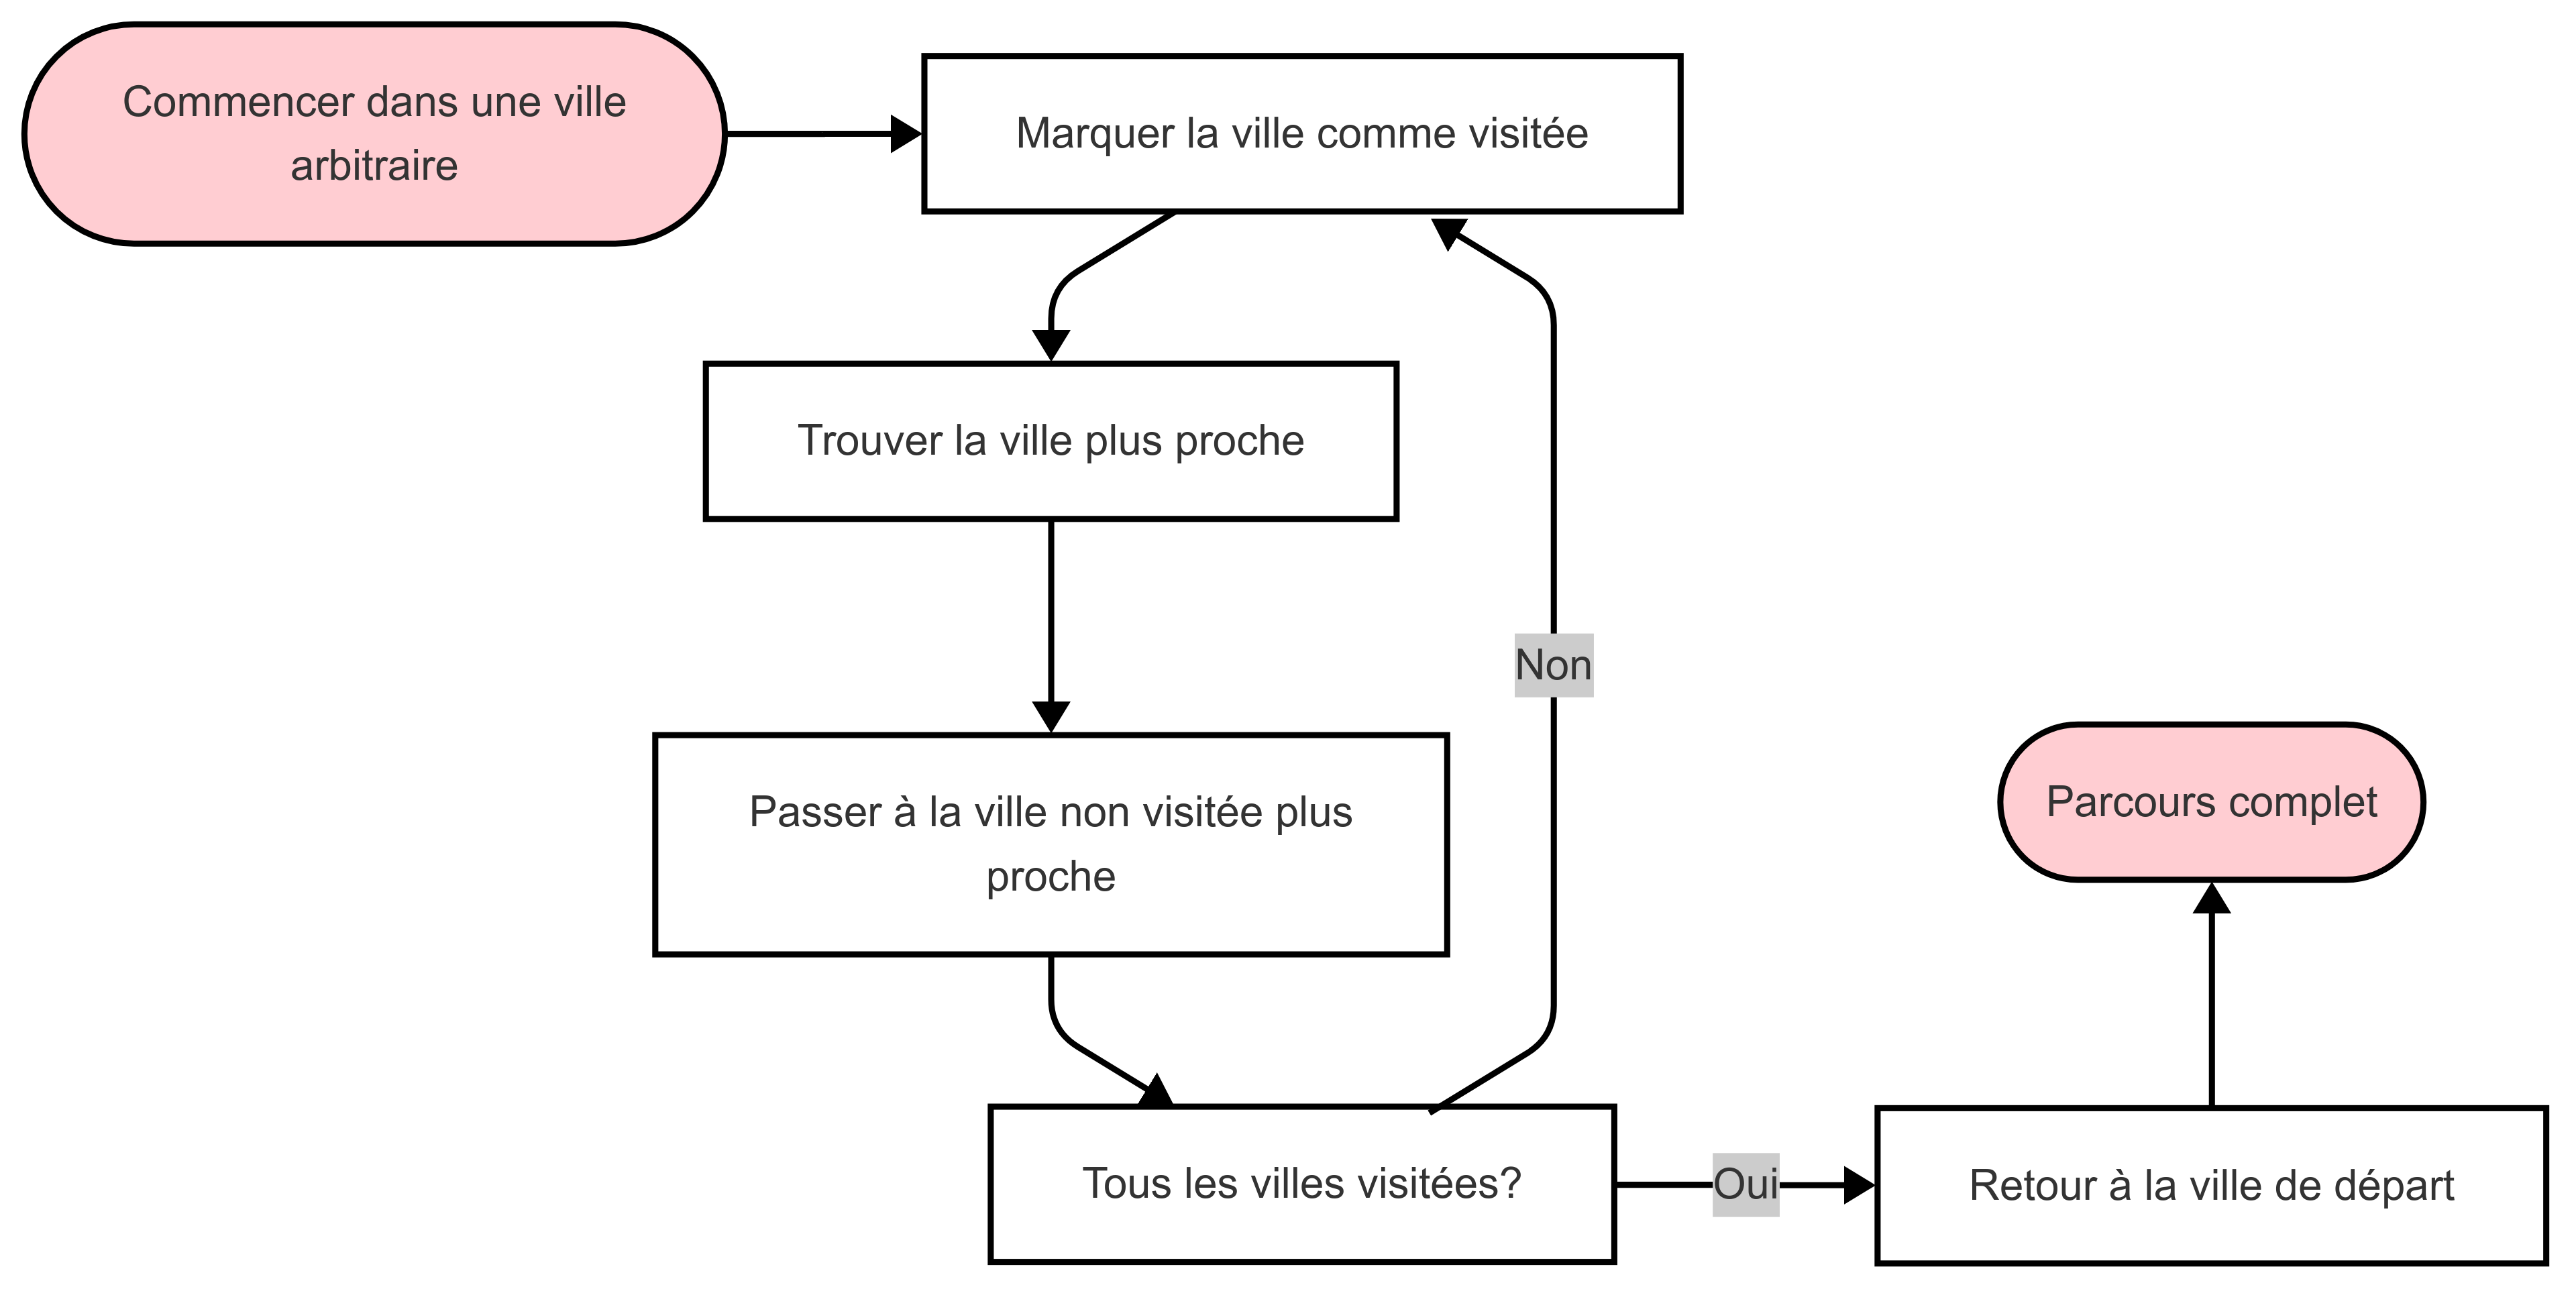
\includegraphics[width=0.7\textwidth]{images/chart-nn.png}
    \caption{Diagramme de l'algorithme.}
    \label{fig:charte-nn}
\end{figure}

\subsection*{Heuristique d’Insertion}
Consiste à assembler un chemin en insérant à chaque étape la ville qui perturbe le moins possible le parcours déjà mis en place. 

\begin{figure}[H]
    \centering
    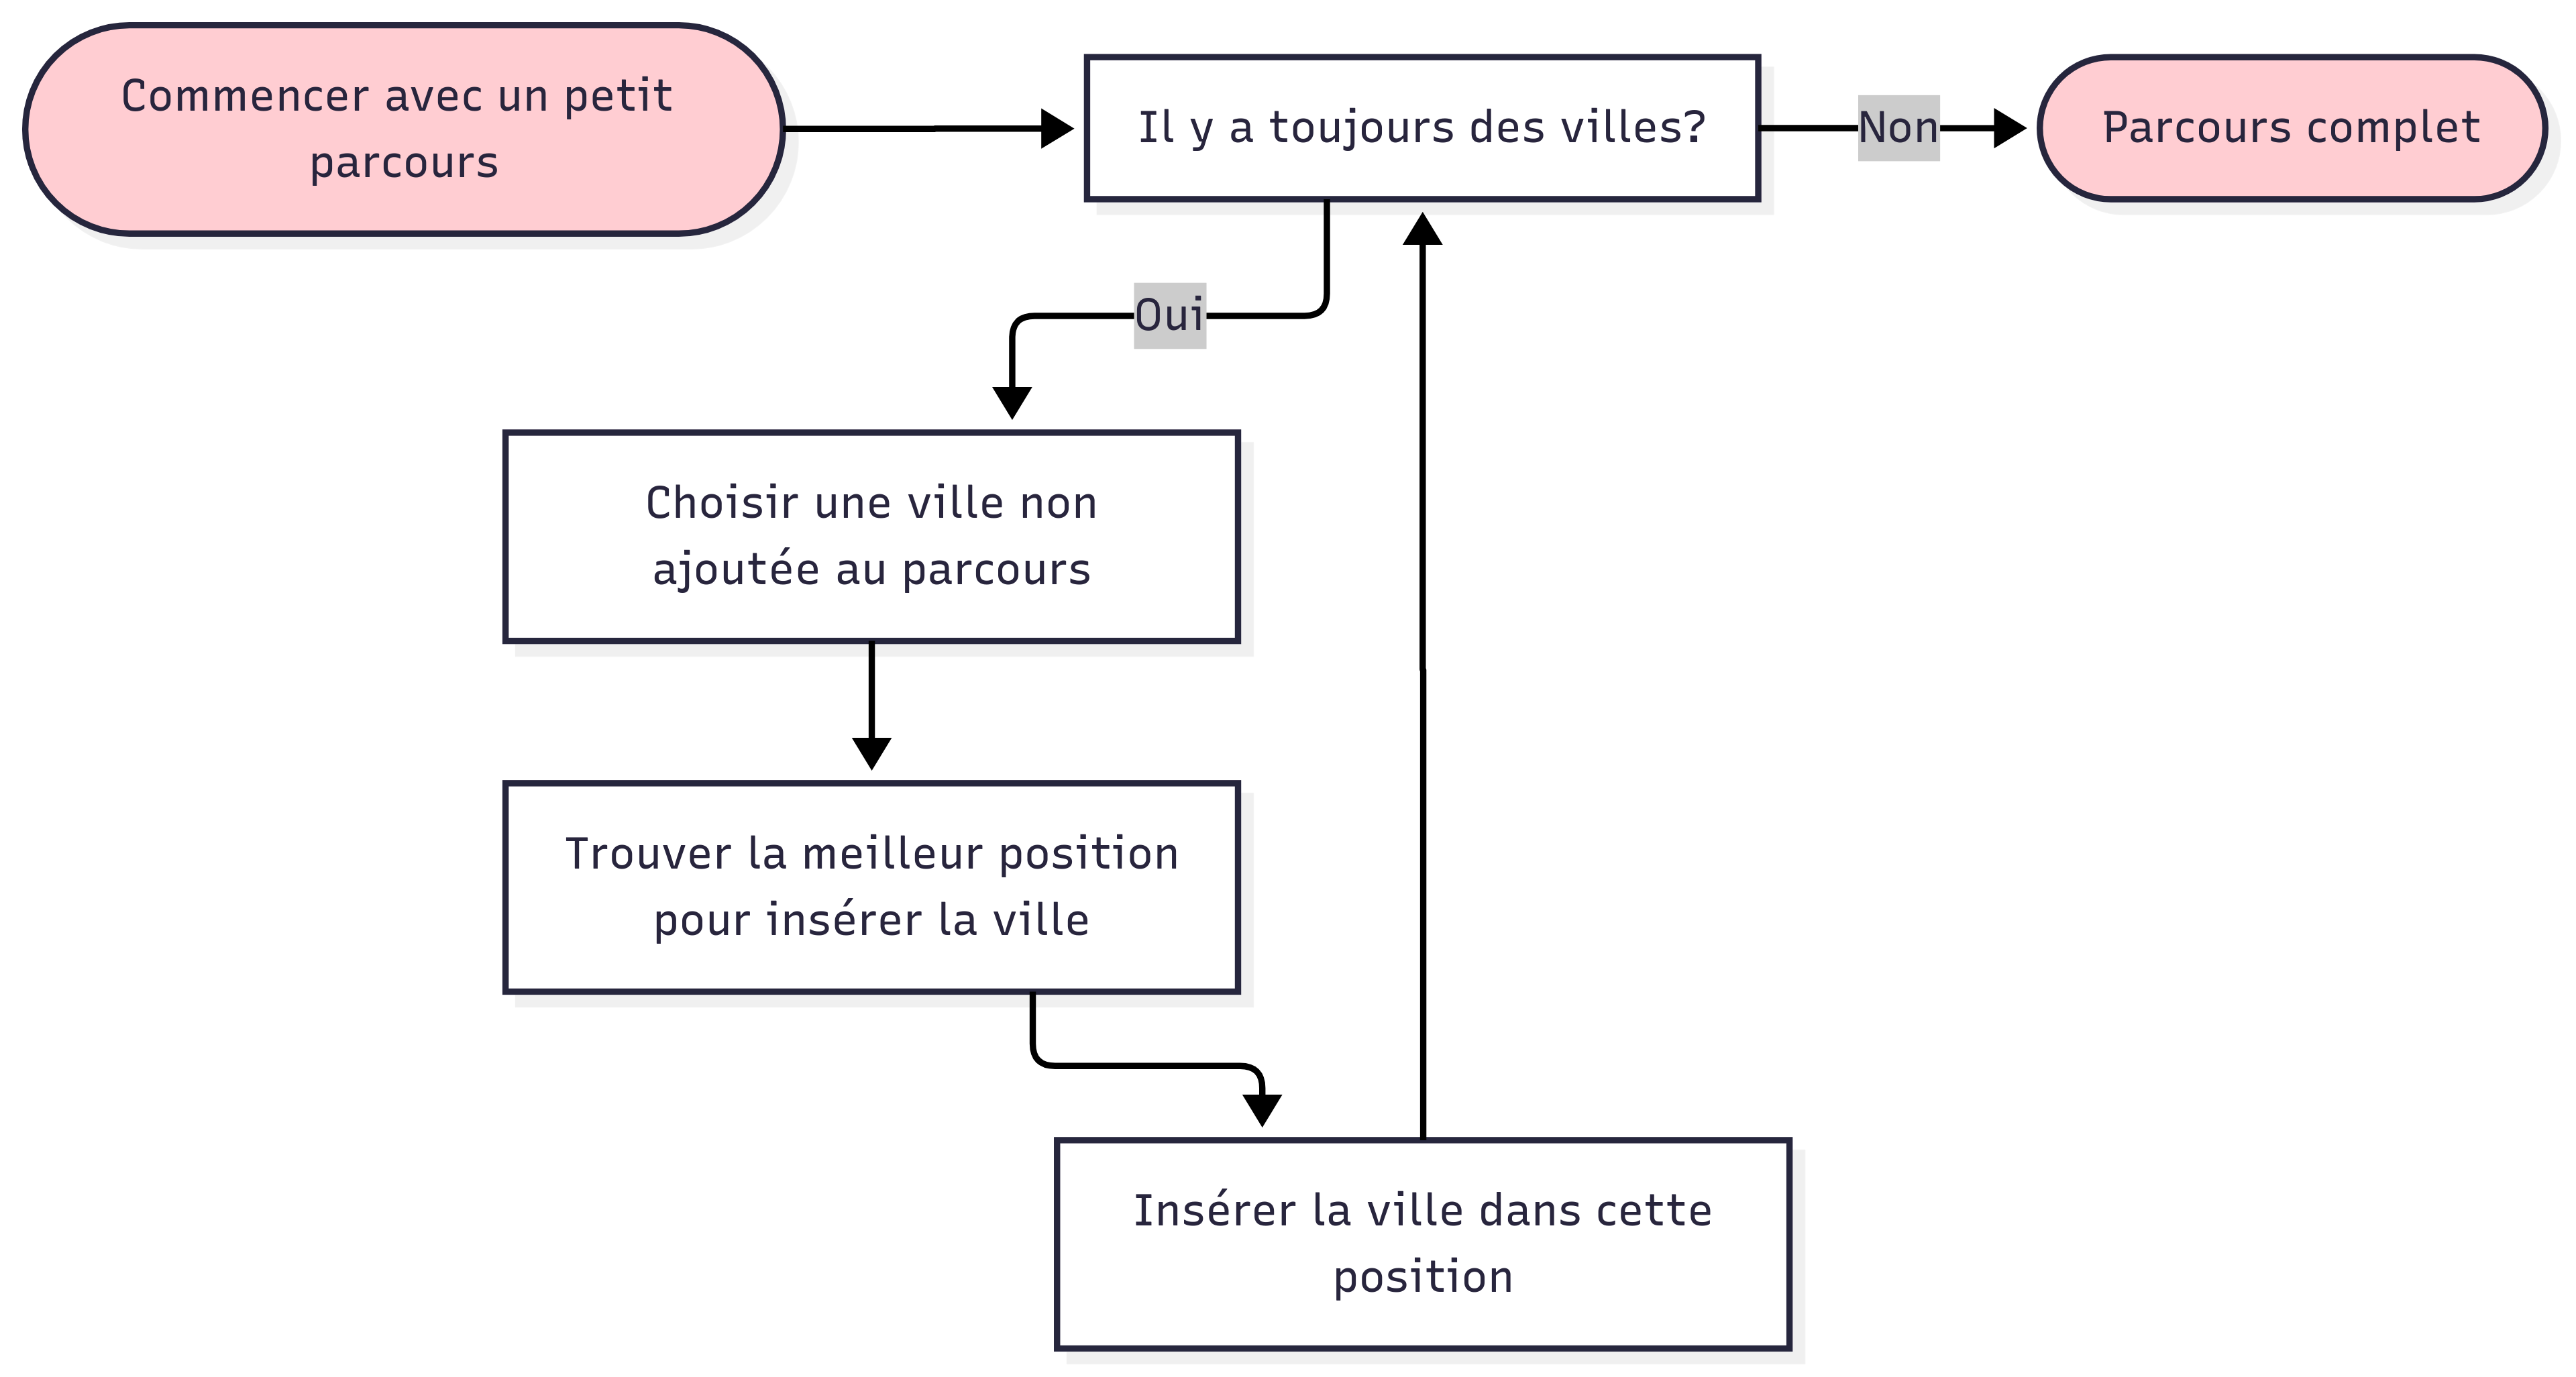
\includegraphics[width=0.7\textwidth]{images/charte-insert.png}
    \caption{Diagramme de l'algorithme.}
    \label{fig:charte-insert}
\end{figure}

\subsection*{2-opt}
L'heuristique 2-opt \cite{article:2opt} est aussi une procédure simplifiée pour chercher le chemin plus optimal. Pour un chemin donné, l'algorithme cherche améliorer le parcours en inversent des sous-chemins. Donc pour chaque ville, l'algorithme cherche le parcours à suivre et vérifie si la distance totale est réduite quand on inverse une partie parcourue. Si l'on trouve un parcours plus court, on garde ce nouveau chemin et commence une fois encore à partir de la ville suivante, et on répète jusqu'à trouver le chemin optimal. La quantité de sous chemins à vérifier est sous-quadratique, mais chaque sous-chemin a une quantité différente de villes, donc la complexité de l'algorithme peut exploser facilement.

\begin{figure}[H]
    \centering
    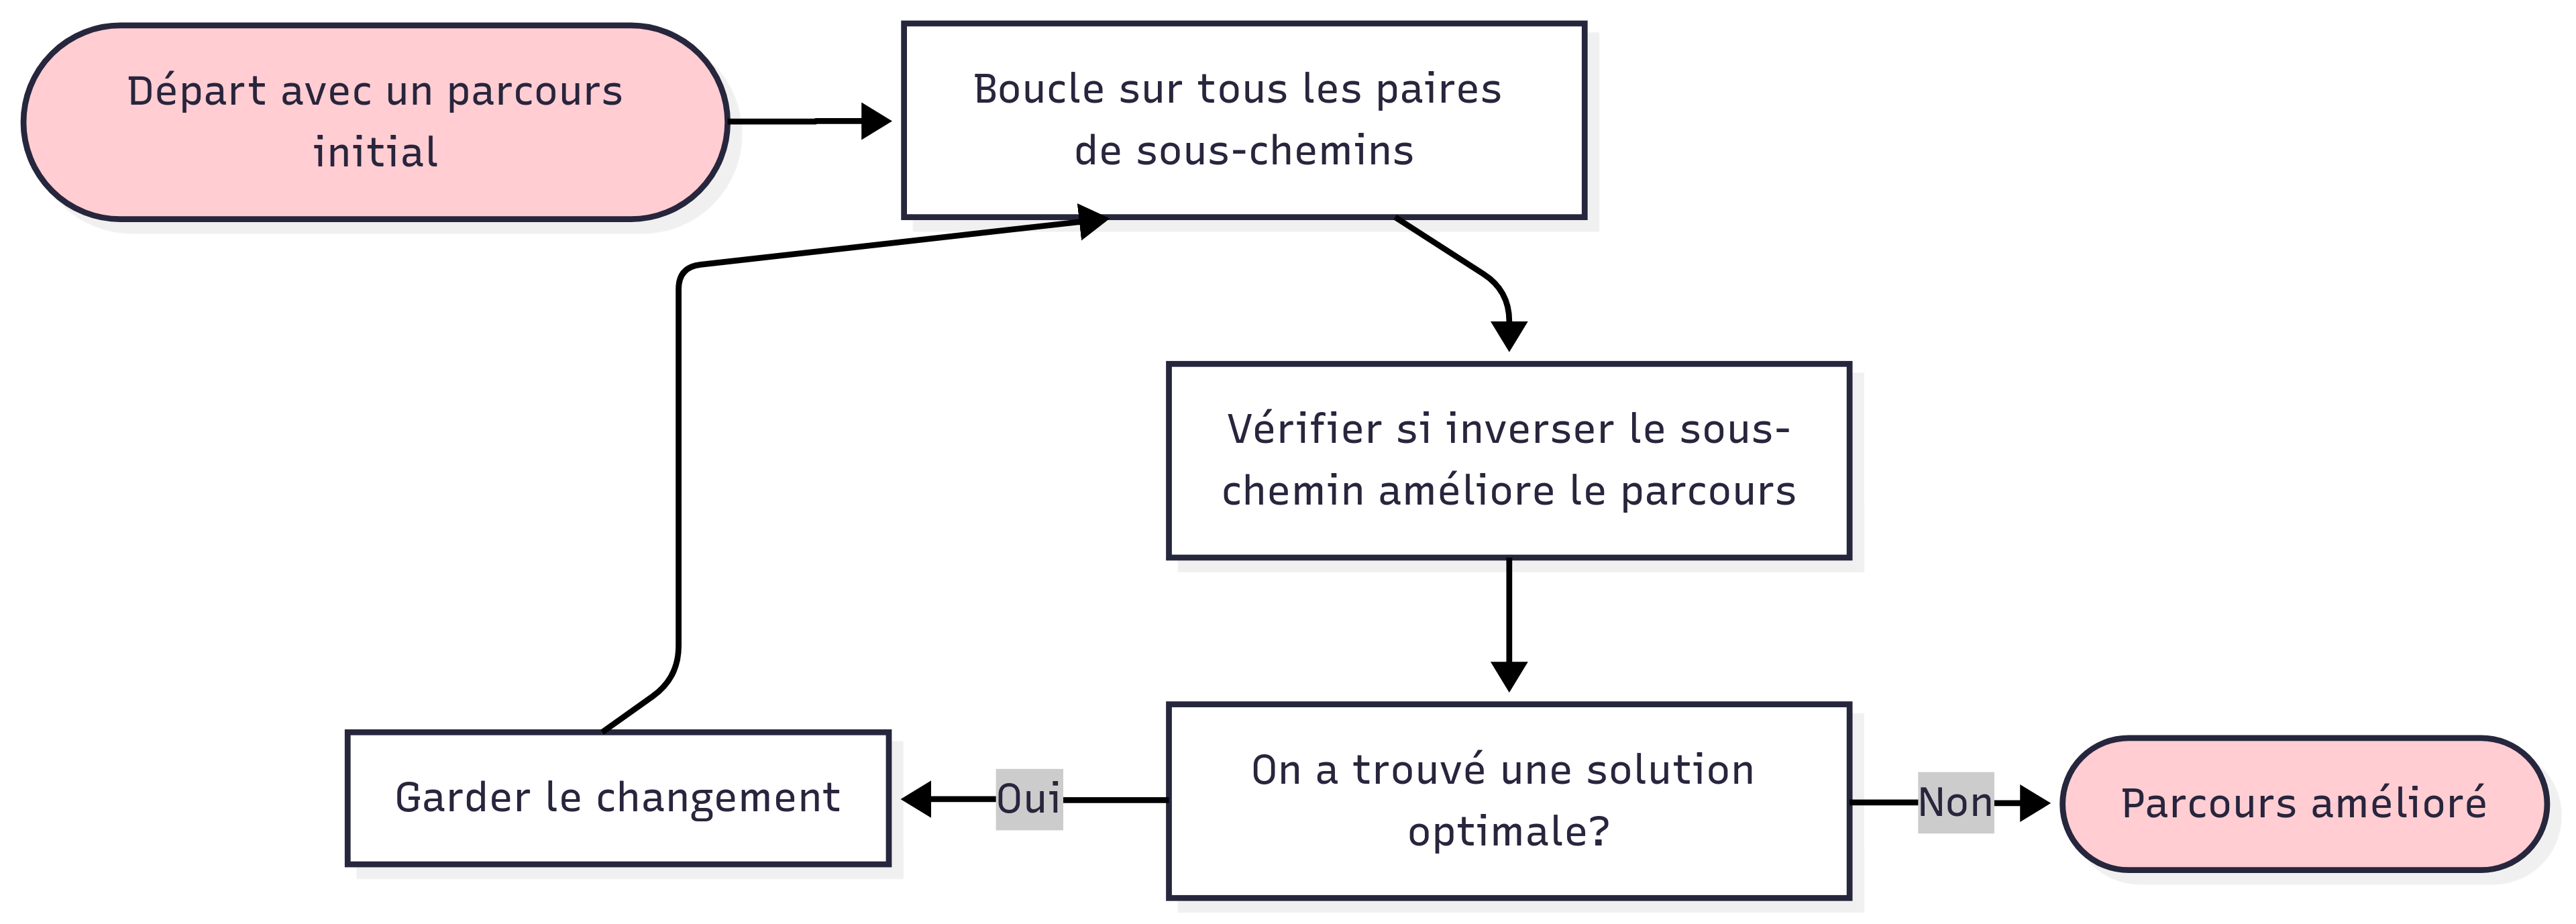
\includegraphics[width=0.8\textwidth]{images/chart-2opt.png}
    \caption{Diagramme de l'algorithme.}
    \label{fig:charte-2opt}
\end{figure}

\subsection*{Recuit Simulé}
Consiste à utiliser une solution déjà proposée et à l’améliorer en utilisant des solutions temporaires qui ne sont pas optimales pour éviter les minima-locaux. 

\begin{figure}[H]
    \centering
    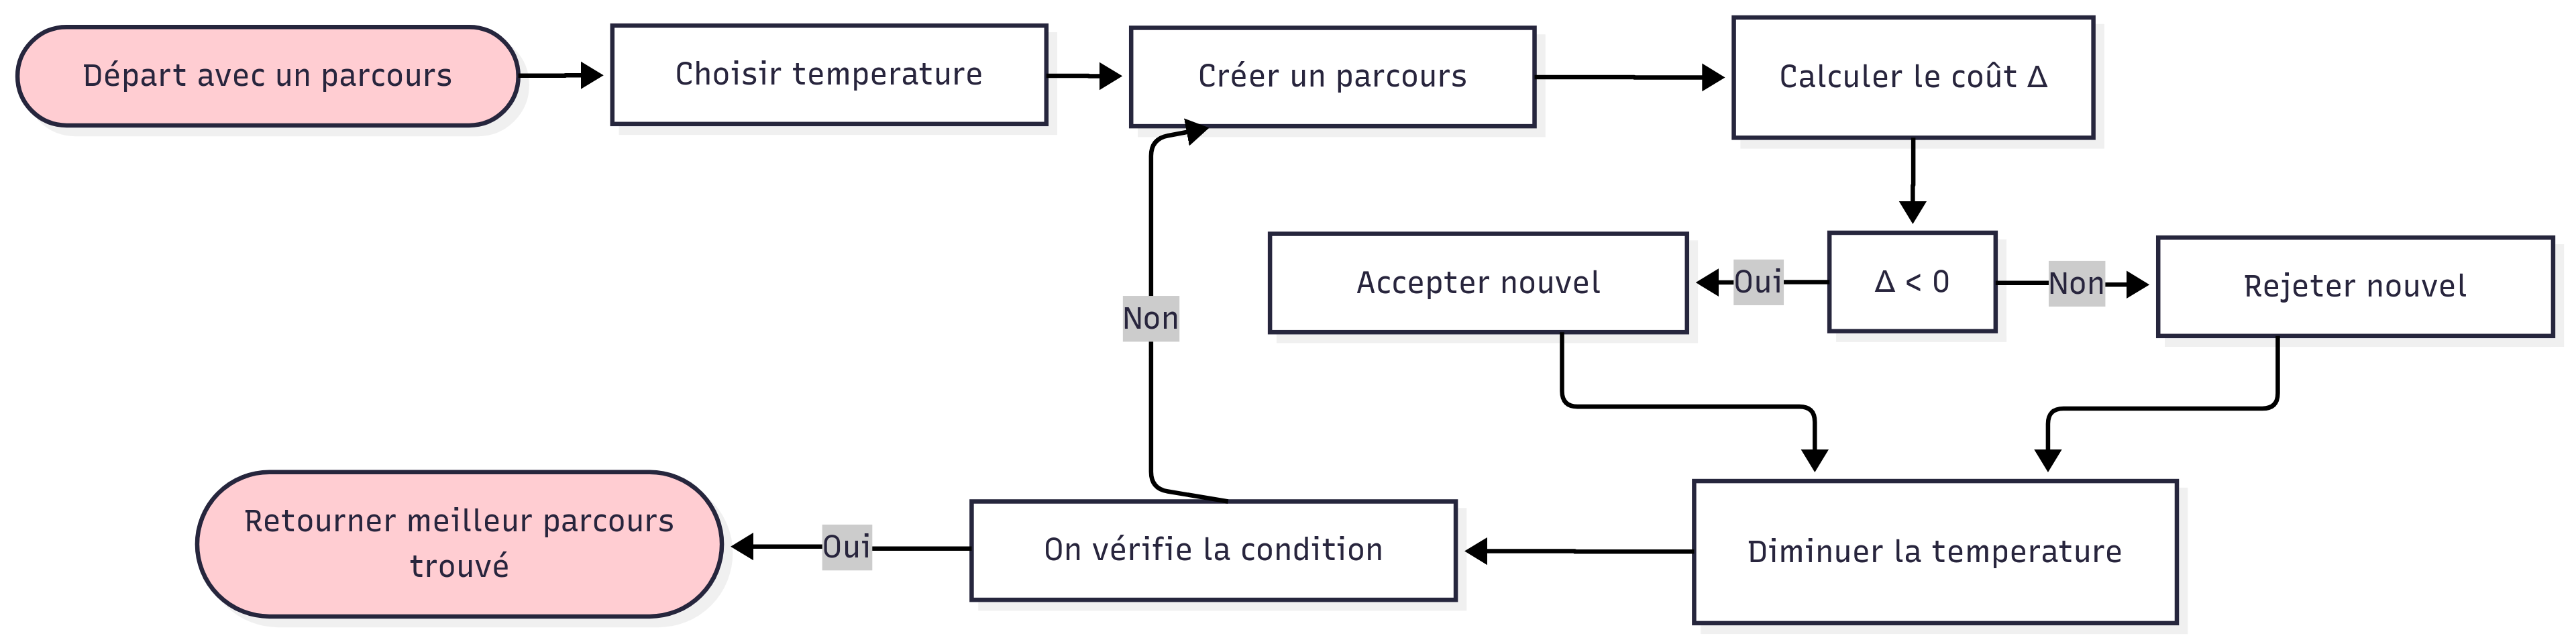
\includegraphics[width=\textwidth]{images/charte-recuit.png}
    \caption{Diagramme de l'algorithme.}
    \label{fig:charte-recuit}
\end{figure}

\section*{\underline{Résultats}}
Voici on présente les résultats obtenus de l'application des algorithmes dans des réseaux de villes. Le code est organisé de façon que on peut donner une graine aléatoire qui génère toujours le même réseau, ce que facilite les comparaisons entre algorithmes.

\subsection*{Voisins plus proches}
Pour essayer l'algorithme des voisins plus proches, on génère un réseau de 50 villes avec un graine égale à 30. On utilise l'algorithme avec trois points de départ différentes: la ville 0, 23 et 42:
\begin{figure}[H]
    \centering
    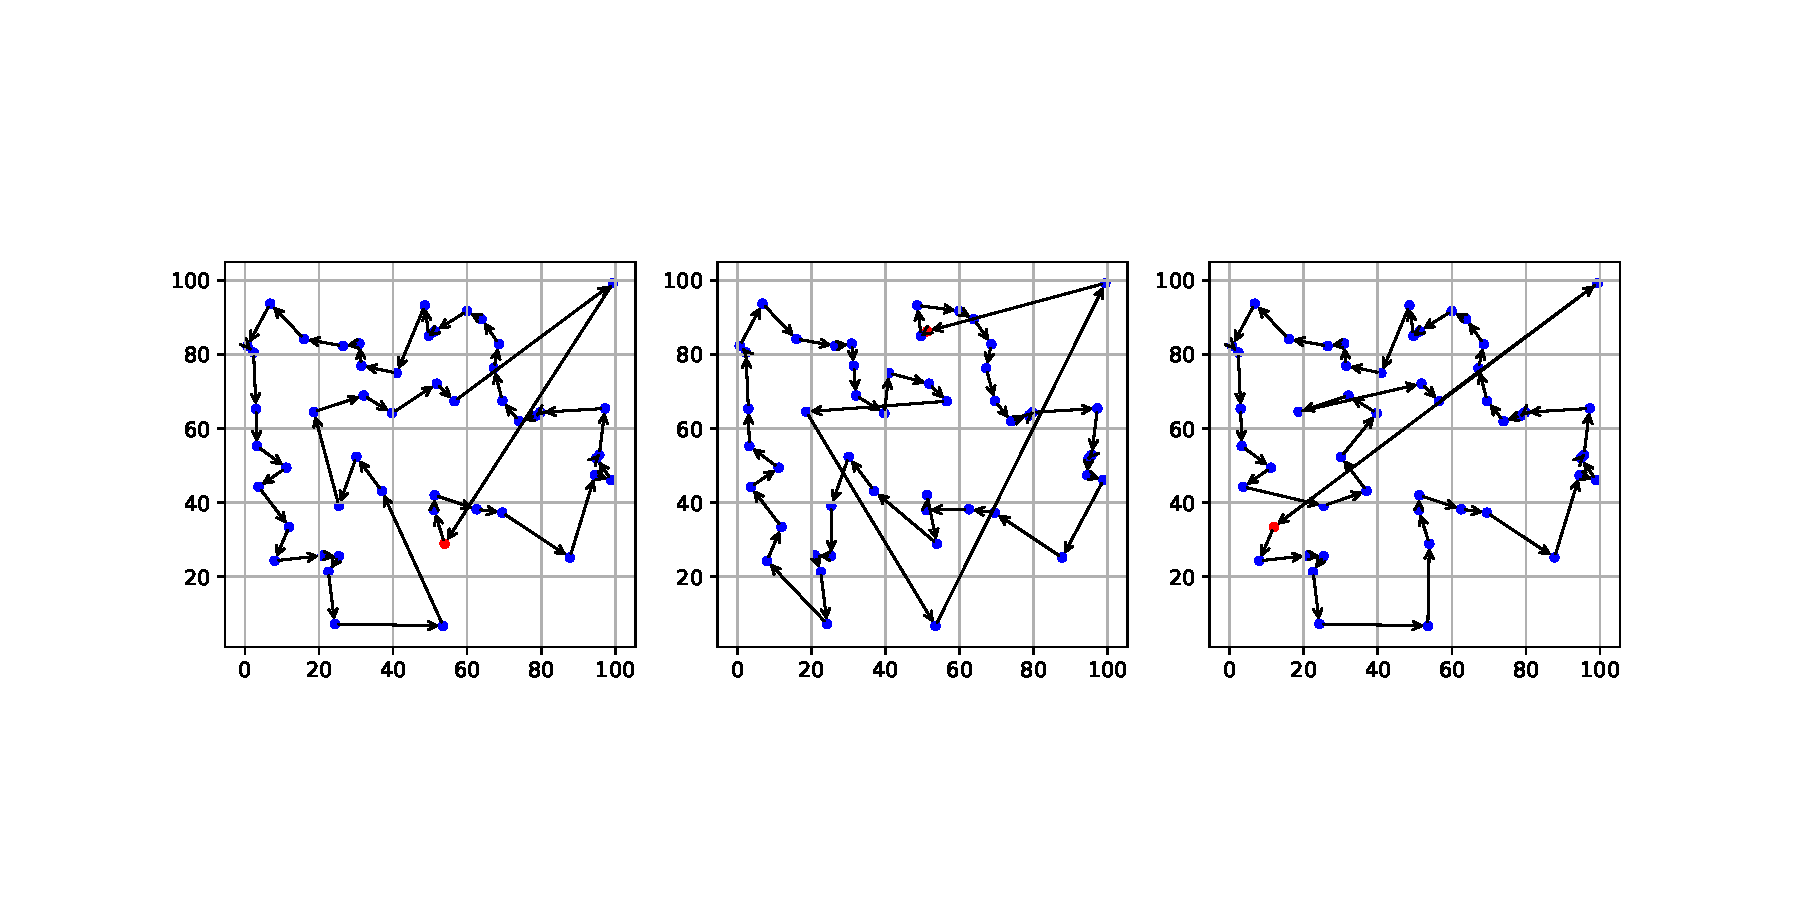
\includegraphics[width=\textwidth]{images/NN_50_villes_3departs.pdf}
    \caption{Résultat pour l'algorithme des Voisins plus proches avec trois départs différents (50 villes). Les départs depuis la ville 0 (gauche), 23 (centre) et 42 (droite).}
    \label{fig:nn-50}
\end{figure}

On a que l'algorithme prendre en moyenne 299.61 microsecondes, et pour chaque point de départ on parcourt:
\begin{itemize}[noitemsep,topsep=5pt]
    \item Départ ville 0 : 669.16.
    \item Départ ville 23 : 715.63.
    \item Départ ville 43 : 692.43.
\end{itemize}

Après ces résultats on peut vérifier que l'optimalité de l'algorithme dépends du point de départ, donc il faudrait appliquer l'heuristique 50 fois pour obtenir la meilleure solution possible avec cet algorithme. En particulier on a une ville qui est trop loin des autres, et cela cause de problèmes avec l'optimalité du chemin parcouru (elle génère croisements dans le chemin).

\subsection*{2-opt}
Pour l'algorithme 2-opt on utilise le même réseau que dans l'heuristique précédent, pour comparer les résultats, avec un départ de la ville 0. Si pour les voisins proches on avait une distance totale de 669.16, avec l'algorithme 2-opt on réduit cette distance à 610.09. Si l'on regarde la Figure \ref{fig:2opt-nn} on voit que cela et dû à l'élimination des croisements, en obtenant un parcours plus direct. Cependant, on a que l'algorithme 2-opt est plus lent. Dans cet exemple, on obtient un temps d'exécution de 71.25 millisecondes, qui est trois ordres de magnitude plus grand.

\begin{figure}[H]
    \centering
    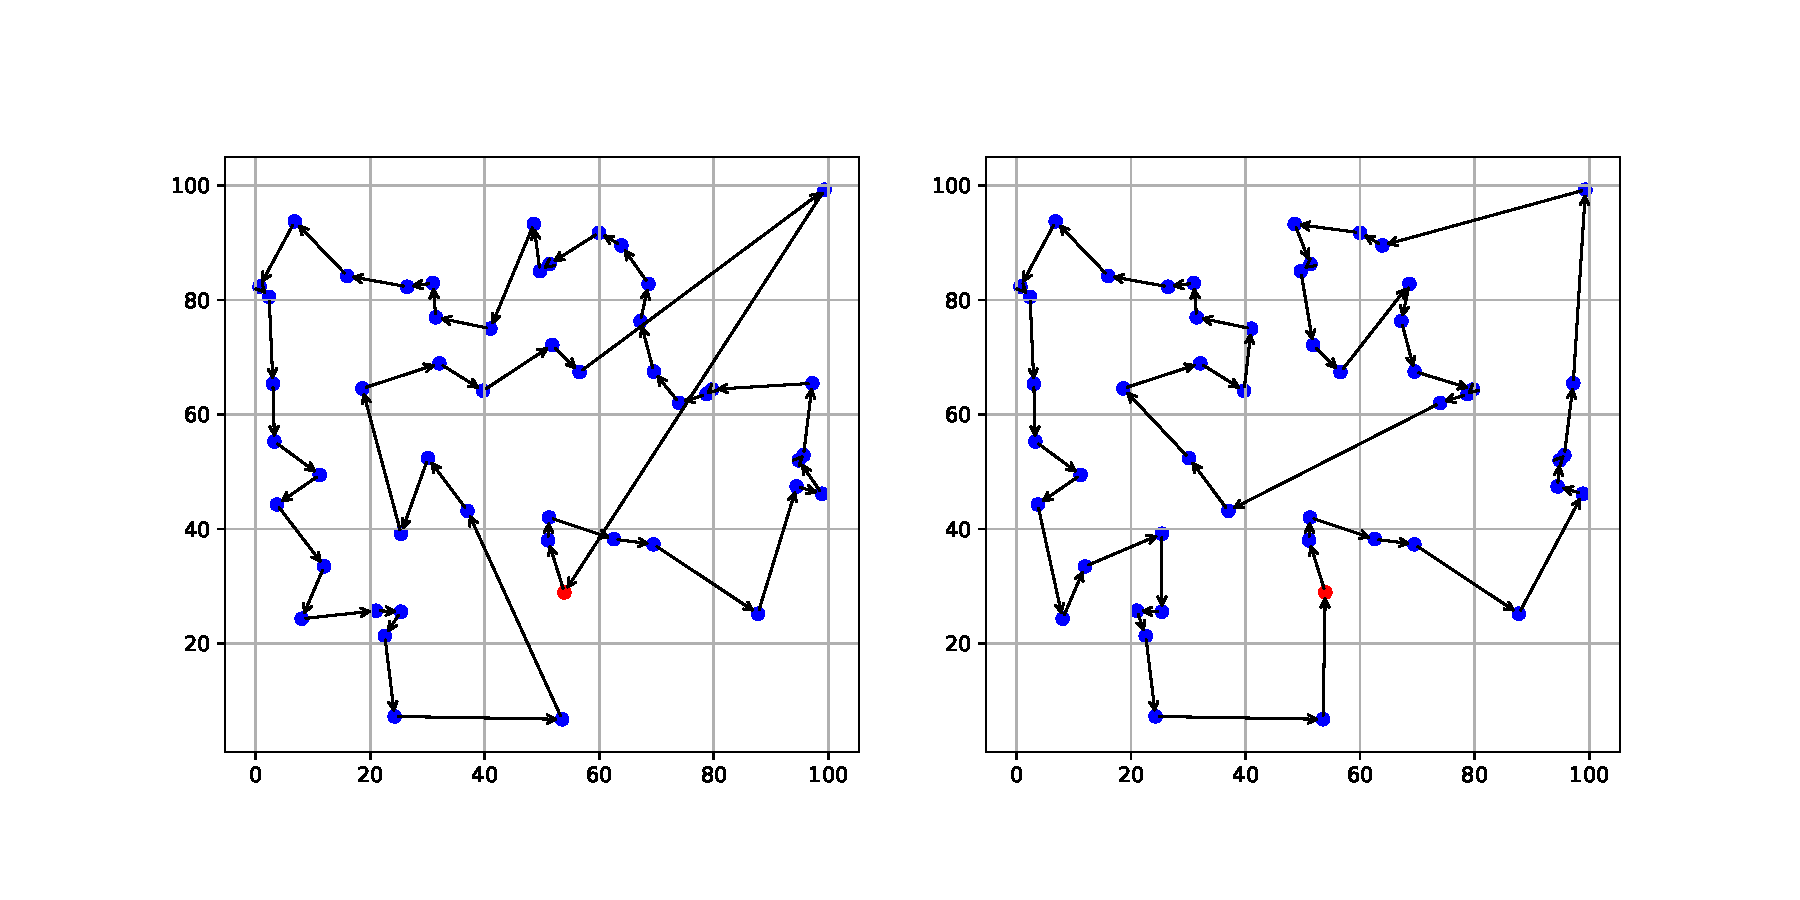
\includegraphics[width=\textwidth]{images/2opt_50_villes_nn.pdf}
    \caption{Résultat pour l'algorithme 2-opt (gauche) et sa comparaison avec le résultat des Voisins plus proches (droite) pour 50 villes.}
    \label{fig:2opt-nn}
\end{figure}

Si l'on applique l'heuristique 2-opt avec une autre solution de voisins plus proches (dans ce cas le même réseau avec départ du ville 23) on a que la distance diminue de 715.63 à 607.72 mais le parcours et différent, ce que nous dit que l'optimalité de l'algorithme 2-opt aussi dépends de son initialisation.

\begin{figure}[H]
    \centering
    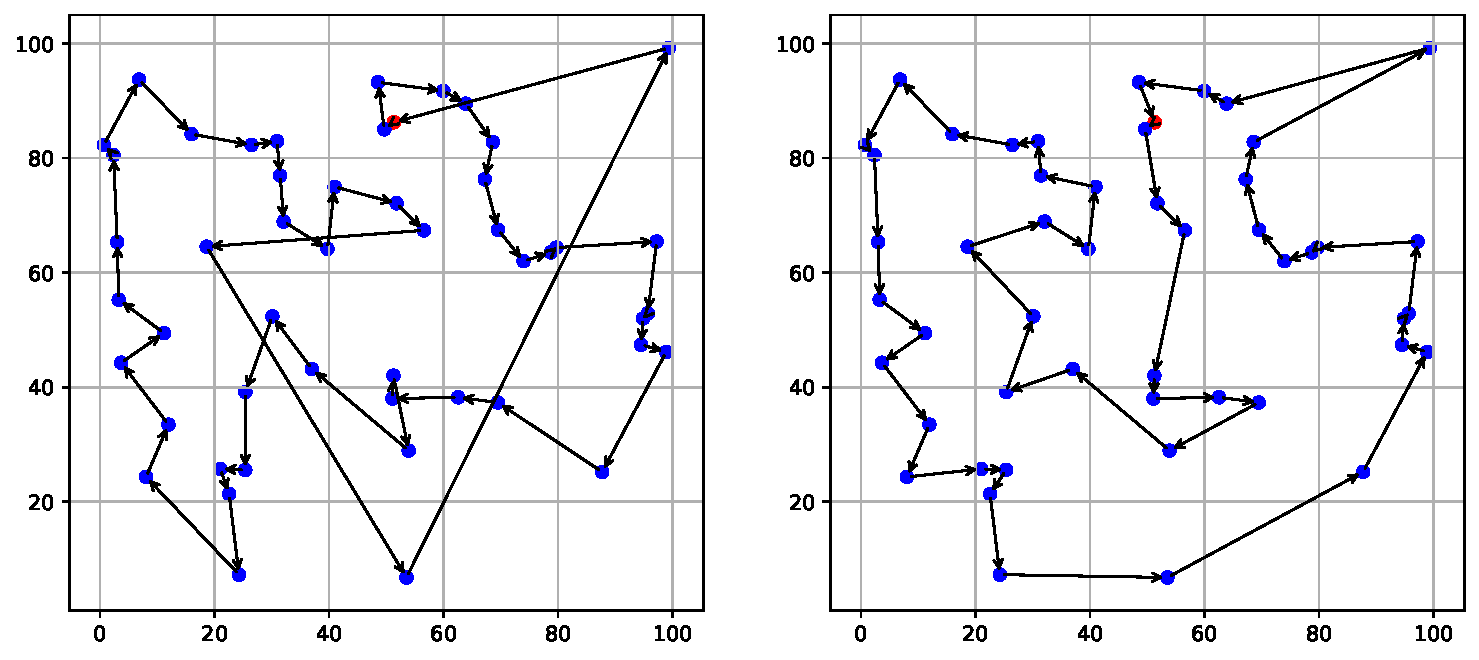
\includegraphics[width=\textwidth]{images/2opt_50_villes_depart_23.pdf}
    \caption{Résultat de 2-opt et sa comparaison avec le résultat des Voisins plus proches pour un départ au milieu.}
    \label{fig:2opt-dep23}
\end{figure}

Finalement, si l'on prendre le parcours avec début dans la ville 42, on a une diminution de la distance parcourue de 692.44 à 609.91, avec l'élimination du grand croisement entre les deux dernières villes.

\begin{figure}[H]
    \centering
    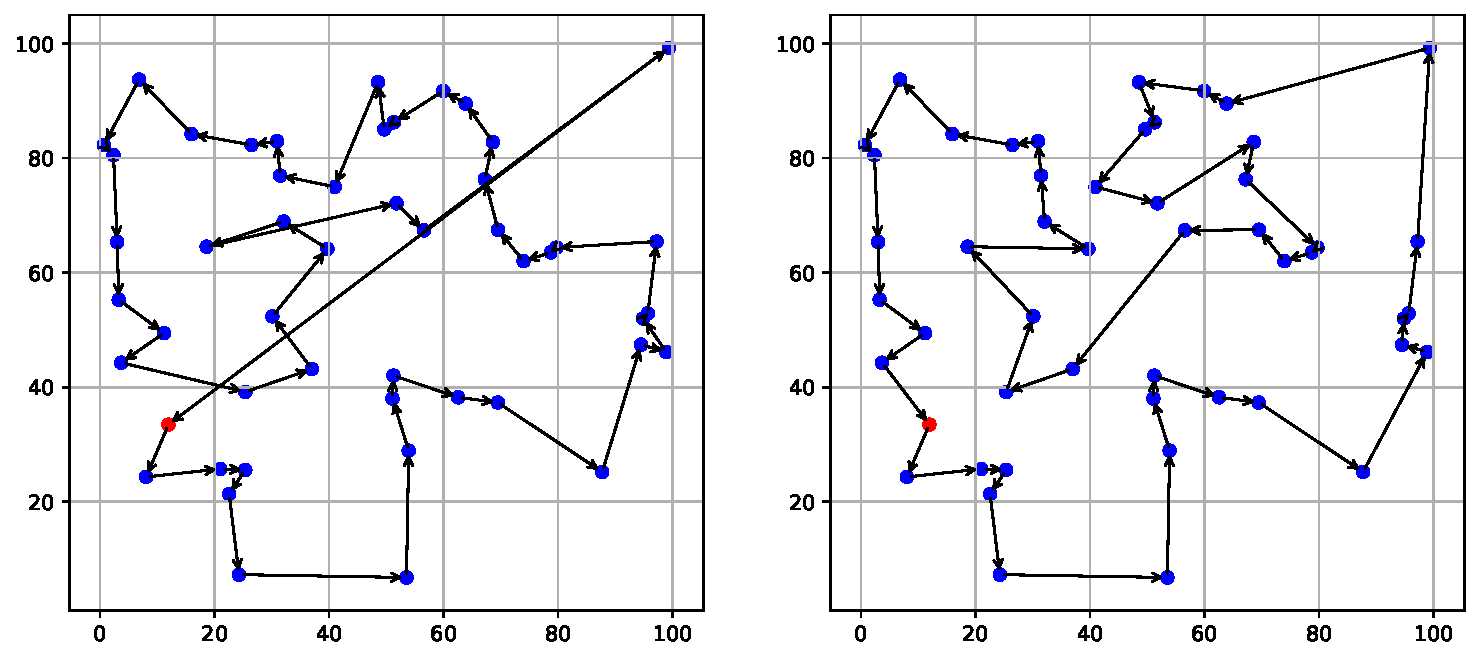
\includegraphics[width=\textwidth]{images/2opt_50_villes_depart_42.pdf}
    \caption{Résultat de 2-opt pour un départ différent. On vérifie que le résultat de 2-opt est dépendent du résultat initial des voisins plus proches, donc le résultat n'est pas fixé.}
    \label{fig:2opt-dep42}
\end{figure}

\subsection*{Heuristique d'insertion}
\paragraph{}
Pour l'heuristique d'insertion avec 20 villes, on obtient un graphe fluide avec une distance totale de 355.04 pour un temps de calcul de 535 microsecondes, que l'on voit sur la Figure \ref{fig:insert-20}
\begin{figure}[H]
    \centering
    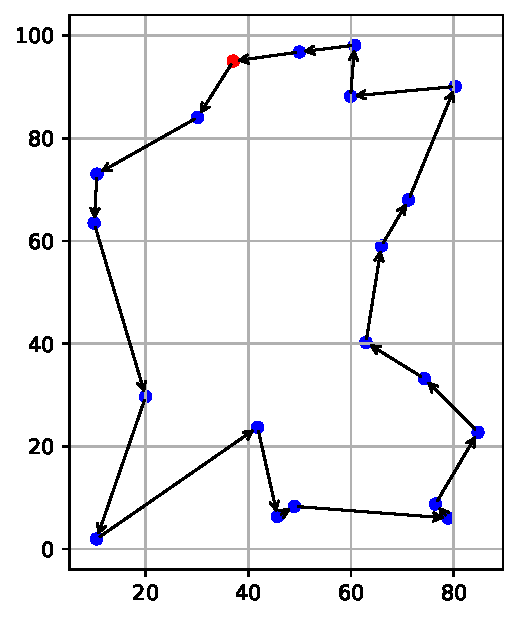
\includegraphics[width=0.35\textwidth]{images/insertion_20_villes.pdf}
    \caption{Résultat pour l'heuristique d'insertion avec 20 villes.}
    \label{fig:insert-20}
\end{figure}
\paragraph{}

Les résultats obtenus pour l'heuristique d'insertion avec 100 villes sont les suivants 

\begin{itemize}[noitemsep,topsep=5pt]
    \item distance totale : 930.16,
    \item temps de calcul : 24.143 millisecondes,
\end{itemize}

tandis que les résultats pour l'heuristique de voisins plus proches sont :

\begin{itemize}[noitemsep,topsep=5pt]
    \item distance totale : 1062.79,
    \item temps de calcul : 0.609 millisecondes.
\end{itemize}

L'algorithme VPP est certe plus rapide que le premier mais il prendre aussi un chemin un peu plus long, et comme on peut le voir sur la figure ci-après, l'heuristique d'insertion ne coupe pas le chemin contrairement au VPP ce qui le rend plus agréable à étudier. 

\begin{figure}[H]
    \centering
    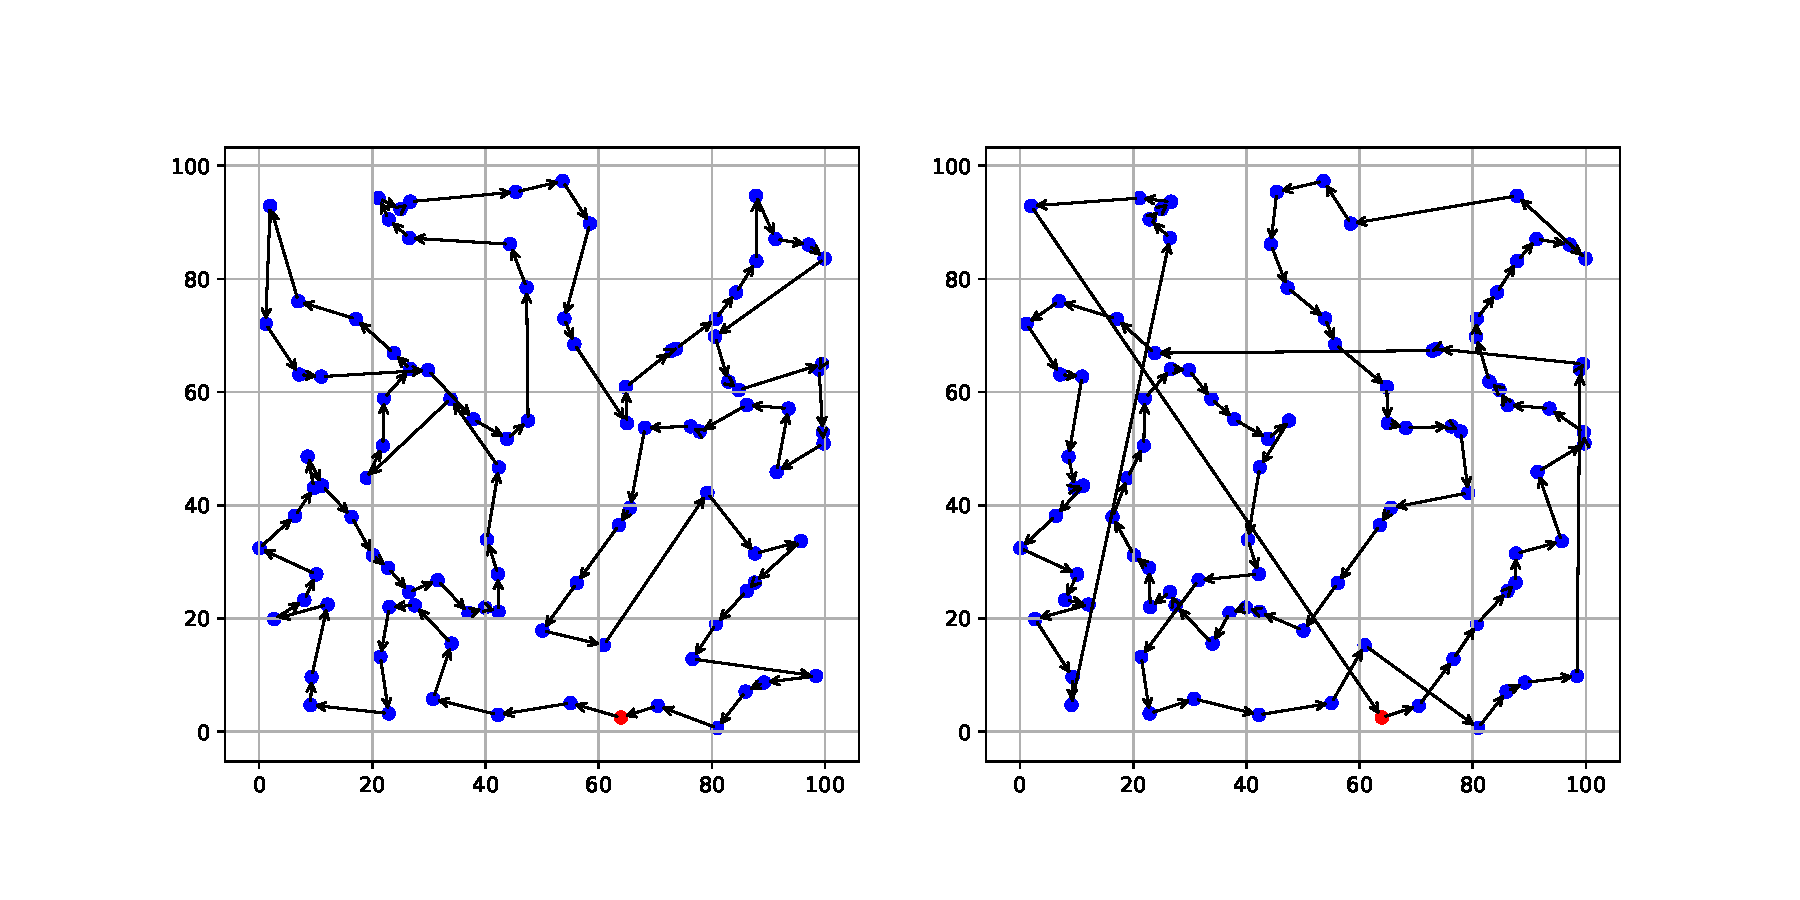
\includegraphics[width=\textwidth]{images/insertion_100_villes_nn.pdf}
    \caption{Résultat pour l'heuristique d'insertion avec 100 villes et une comparaison avec le résultat des Voisins plus proches pour le même réseau.}
    \label{fig:insert-100}
\end{figure}

\subsection*{Recuit simulé}
\paragraph{}
Nous obtenons les mesures suivantes pour l'heuristique d'insertion : 
\begin{itemize}[noitemsep,topsep=5pt]
    \item distance totale : 897.78,
    \item temps de calcul : 31.324 millisecondes,
\end{itemize} 
contre ces résultats pour le recuit simule:
\begin{itemize}[noitemsep,topsep=5pt]
    \item distance totale : 865.26,
    \item temps de calcul : 308.325 millisecondes.
\end{itemize}
Comme on le constate sur la Figure \ref{fig:recuit}, même si le temps de calcul augmente et est multiplié par 10 par rapport à l'heuristique d'insertion, la distance du chemin est diminuée et optimisé. Le temps de calcul reste très faible pour cette quantité de villes : environ 300 millisecondes, ce qui rend le recuit simulé optimal pour des calculs de chemins avec un nombre de villes important.
\begin{figure}[H]
    \centering
    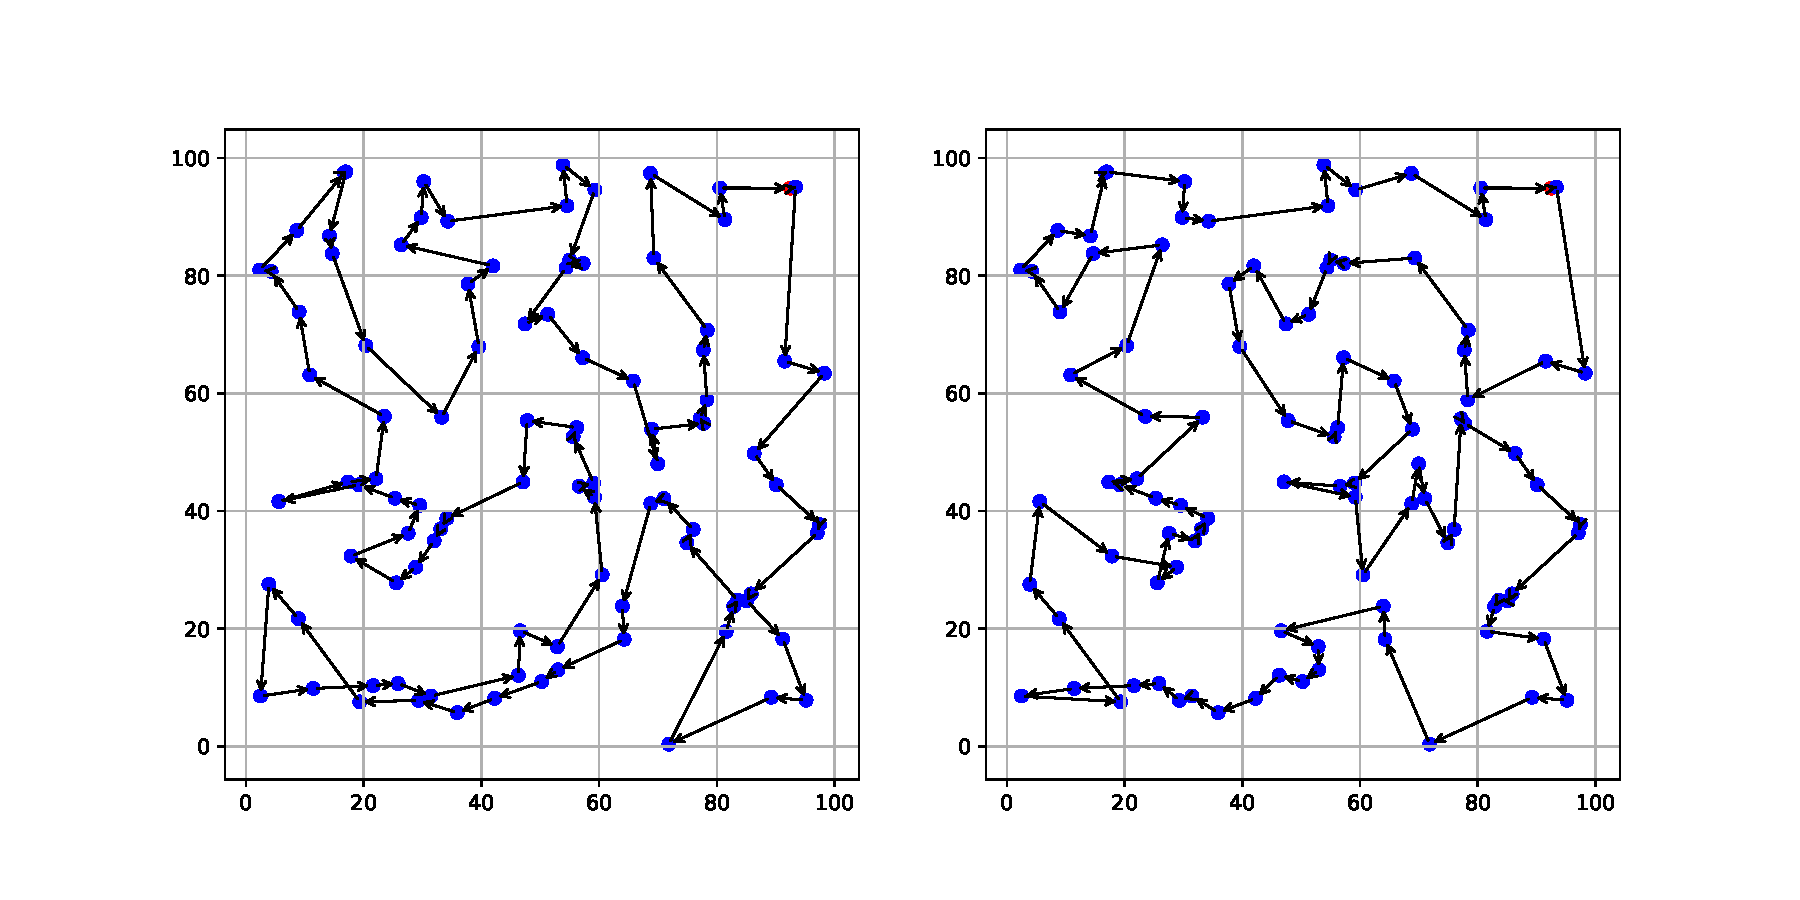
\includegraphics[width=\textwidth]{images/recuit_simule.pdf}
    \caption{Résultat pour l'heuristique d'insertion (à gauche) et son amélioration par l'algorithme de Recuit simulé (à droite) avec 100 villes.}
    \label{fig:recuit}
\end{figure}

\subsection*{Comparaison entre algorithmes}
Les différents algorithmes analysés ont ses avantages et problèmes, mais sauf cas particulières on ne les compare pas directement. Ici, on prendre des réseaux avec un graine choisi aléatoirement (3456) de différentes dimensions : on génère réseaux de 10, 50, 100, 500 et 1000 villes et l'on applique les différents heuristiques pour trouver les meilleures solutions de chaque algorithme. Les résultats sont montrés dans le tableau \ref{tab:distances} : 
\begin{table}[H]
    \centering
    \caption{Distance obtenue avec les différents algorithmes pour une quantité $N$ de villes.}
    \label{tab:distances}
    \begin{tabular}{lcccc}
        \hline
        N villes & VPP & 2-opt & Heuristique d'insertion & Recuit simulé \\ \hline\hline
        10  & 286.2587  & 266.1043  & 299.9325 & 266.1043 \\
        50  & 588.5159  & 549.2188  & 615.9452 & 565.7999 \\
        100 & 888.5622 & - & 853.6044 & 827.6085 \\
        500 & 2099.8537 & - & 1936.8251 & 1936.8251 \\
        1000 & 2916.9891 & - & 2716.844 & 2716.8443  \\ \hline
    \end{tabular}
\end{table}

La première chose à noter est le manque des données pour l'algorithme 2-opt. Cela est dû à l'inefficience de l’algorithme. Pour un réseau de 100 villes l'algorithme ne converge pas après 5 minutes, donc inutile d'attendre car l’incrémente de temps pour les réseaux plus grandes rendra impossible la solution. Cependant, on peut voir que dans les cases ou 2-opt est présente il donne la solution plus optimale au problème pour ce réseau particulier. C'est intéressant de noter aussi que pour les réseaux plus petites l'heuristique d'insertion n'est pas plus optimale que les voisins plus proches, mais avec la croissance des réseaux on a une amélioration de la performance de l'heuristique. Mais comme on a déjà vu, l'algorithme des Voisins plus proches est plus vite, donc est intéressante aussi de faire le compromis entre temps et précision.

\subsection*{Complexité temporelle}
Finalement, on fait une analyse temporelle des algorithmes pour voir la tendance en fonction de la taille des réseaux. Pour ce cas, On utilise les algorithmes pour résoudre le TSP pour réseaux de 10, 50, 100, 500 et 1000 villes, mais cette fois-ci on génère des réseaux aléatoires et pour chaque taille on résoudre le problème 5 fois, pour avoir une signifiance statistique. Les résultats sont visibles dans la Figure \ref{fig:temps} :

\begin{figure}[H]
    \centering
    
\includegraphics[width=0.65\textwidth]{images/complexite_temporelle.pdf}
    \caption{Nombre de villes vs. le temps moyenne d'exécution des algorithmes.}
    \label{fig:temps}
\end{figure}

On montre les courbes dans un espace logarithmique pour faire une régression polynomiale qui permettre d'obtenir une droite pour chaque courbe. Ces droites ont pour pente :

\begin{itemize}
    \item Voisins plus proches : 1.636,
    \item Heuristique d'insertion : 2.902,
    \item Recuit simulé : 0.721.
\end{itemize}

On peut voir que l'algorithme de voisins plus proches, pour les cas que l'on a analysé a une complexité de $\mathcal{O}(n^{1.636})$, qui est dans l'ordre de magnitude de $n^2$, le pire cas. Pour l'heuristique d'insertion on obtient $\mathcal{O}(n^{2.902})$ qui est pire que le $n^2$ attendu, mais dans une marge acceptable. Finalement, on voit que le Recuit simulé donne une complexité $\mathcal{O}(n^{0.721})$, qui est très efficient en comparaison aux autres algorithmes. On peut attendre que pour des réseaux très grandes il serait l'option la plus avantageuse, mais il faut considérer quand même que pour utiliser cette stratégie il faut utiliser un autre heuristique avant pour démarrer l'analyse.

\newpage

\section*{\underline{Conclusion}}
Résumé travail

Résumé résultats

Problèmes et challenges

Comment améliorer à futur

\newpage
\bibliographystyle{unsrt}
\bibliography{bibliography}

\end{document}

